\subsection{Butterfly parametric equation}
\begin{table}[ht]
	\begin{center}
		\begin{tabular}[top]{ |p{16.0 cm}| }
			\rowcolor{LIGHTCYAN}			
			%% \hline \multicolumn{1}{|c|}{\textbf{Part 1/5 Teardrop and Butterfly parametric curves}} \\ [1.0ex]
	
			\rowcolor{LIGHTCYAN}
			\hline \textbf{No. 2 - Butterfly parametric curve}\\
			\begin{eqnarray}
				x(u) & = & \sin(2\pi u) \left [ e^{\cos(2\pi u)} - 2\cos(8\pi u) - (\sin(2\pi u/12))^5 \right] \nonumber \\
				y(u) & = & \cos(2\pi u) \left [ e^{\cos(2\pi u)} - 2\cos(8\pi u) - (\sin(2\pi u/12))^5 \right] \nonumber \\
				u & \in & [0.0, 1.0] \nonumber
			\end{eqnarray}
			      
			
			Closed loop\\
			Overall Multiple loops\\
			Reflection x-axis: non-symmetrical\\
			Reflection y-axis: symmetrical\\
			\frame{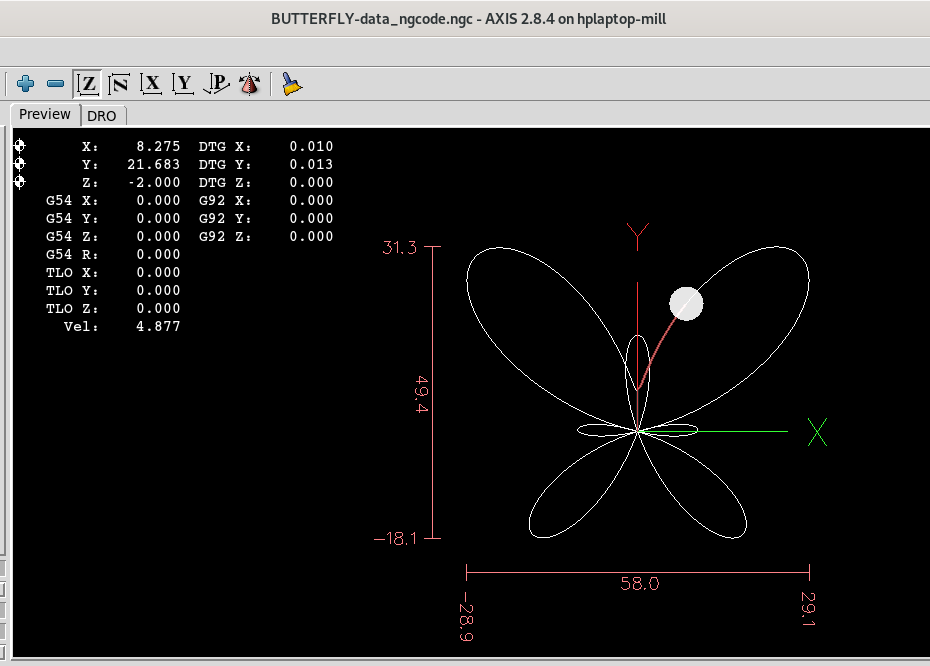
\includegraphics[width=0.56\textwidth]{./07-images/img-Ch5/BUTTERFLY-Axis.png}}
            \frame{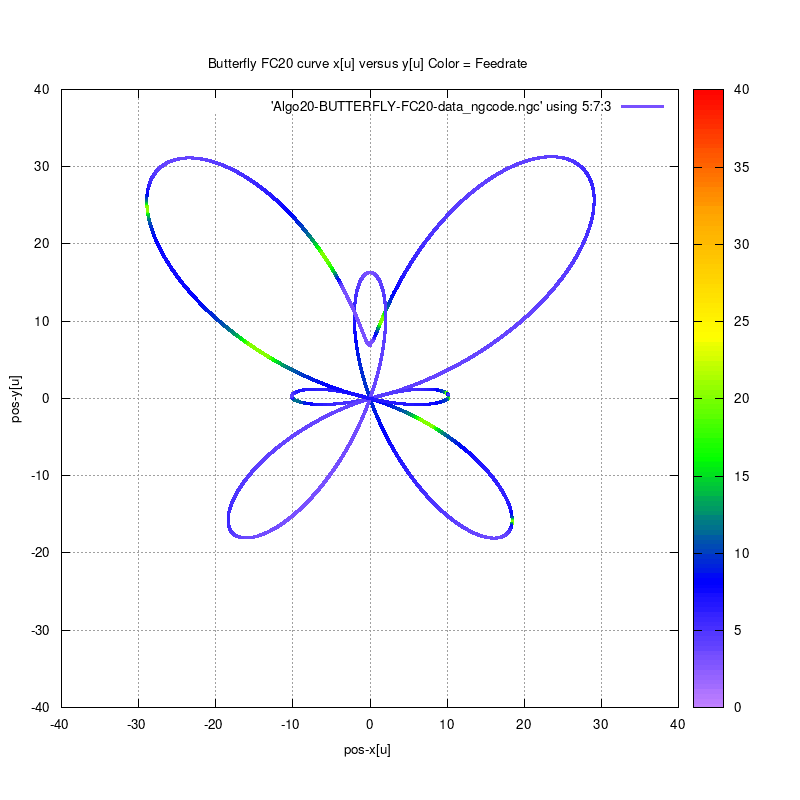
\includegraphics[width=0.40\textwidth]{./07-images/img-Ch5/BUTTERFLY-Feedrate.png}}\\

			\hline
		\end{tabular}
		\caption{Butterfly parametric equation and dimensions}		
		\label{table:Butterfly parametric equation}
	\end{center}
\end{table}  
